\documentclass[10pt,reqno, final]{amsart}
\usepackage[notcite,notref]{showkeys}

\usepackage{url,hyperref,multirow}
\usepackage{color}
\usepackage{stmaryrd}
\usepackage{exscale}

\usepackage{relsize}

\usepackage{epsfig,subfigure,amssymb,amsmath,version,slashbox}
\usepackage{amssymb,version,graphicx,fancybox,mathrsfs,pifont,booktabs}%,wrapfig}

\usepackage{epstopdf}
%\usepackage[active]{srcltx}

%\textwidth 6in
% \textheight 8in
%\renewcommand{\baselinestretch}{1.2}
\usepackage{graphicx}

\headheight=3pt
\topmargin=0.3cm
\textheight=8.5in
\textwidth=5.8in
\setlength{\oddsidemargin}{1cm}
\setlength{\evensidemargin}{1cm}
\addtolength{\voffset}{-5pt}

\catcode`\@=11 \theoremstyle{plain}
%\@addtoreset{equation}{section}   % Makes \section reset 'equation' counter.
%\renewcommand{\theequation}{\arabic{section}.\arabic{equation}}
%\@addtoreset{figure}{section}
%\renewcommand\thefigure{\thesection.\@arabic\c@figure}
%\@addtoreset{table}{section}
%\renewcommand\thetable{\thesection.\@arabic\c@table}


\renewcommand{\theequation}{\thesection.\arabic{equation}}
\newtheorem{lemma}{Lemma}[section]
\newtheorem{theorem}{Theorem}[section]
\newtheorem{corollary}{Corollary}[section]
\newtheorem{proposition}{Proposition}[section]
\newtheorem{definition}{Definition}[section]
\newtheorem{remark}{Remark}[section]
\newtheorem{example}{Example}[section]
\@addtoreset{figure}{section}
\renewcommand\thefigure{\thesection.\@arabic\c@figure}
\@addtoreset{table}{section}
\renewcommand\thetable{\thesection.\@arabic\c@table}




\newcommand{\bs}[1]{\boldsymbol{#1}}
\def \ri {{\rm i}}



\newcommand{\comm}[1]{\marginpar{%
\vskip-\baselineskip %raise the marginpar a bit
\raggedright\footnotesize
\itshape\hrule\smallskip#1\par\smallskip\hrule}}

\DeclareSymbolFont{ugmL}{OMX}{mdugm}{m}{n}
\SetSymbolFont{ugmL}{bold}{OMX}{mdugm}{b}{n}

\DeclareMathAccent{\wideparen}{\mathord}{ugmL}{"F3}


%\newcommand{\namelistlabel}[1]{\mbox{#1}\hfill}
%\newenvironment{namelist}[1]{%
%\begin{list}{}
%{
%     \let\makelabel\namelistlabel
%     \settowidth{\labelwidth}{#1}
%     \setlength{\leftmargin}{1.3\labelwidth}
%    }
%  }}%
%\end{list}}
\begin{document}
\bibliographystyle{plain}
\graphicspath{{./figs/}}
\baselineskip 13pt
\title{Hybridizable discontinuous Galerkin method for elliptic problem}
\maketitle
\section{2-D problem}
\subsection{Model problem}
\begin{equation}
\label{modelproblem}
\left\{\begin{array}{ll}\displaystyle -\nabla\cdot\nabla
u(x)=f(x)&\displaystyle x\in\Omega\\
\displaystyle u=g &\displaystyle on\quad \partial\Omega
\end{array}\right.
\end{equation}

\subsection{HDG scheme}
Some notations:
\begin{enumerate}
\item Denote by $\mathcal{T}_h$ a collection of disjoint regular elements $K$ that partition $\Omega$
and set $\partial\mathcal{T}_h:=\{\partial K: K\in\mathcal{T}_h\}$.

\item For an element $K$ of the collection $\mathcal{T}_h$, $F=\partial K\cap\partial\Omega$ is the
boundary face if the $d-1$ Lebesgue measure of $F$ is nonzero. For two elements $K^+$ and $K^-$ of
the collection $\mathcal{T}_h$, $F=\partial K^+\cap\partial K^-$ is the interior face between $K^+$
and $K^-$ if the $d-1$ Lebesgue measure of $F$ is nonzero. Denote by $\mathcal{E}_h^o$ and $\mathcal{E}_h^{\partial}$
the set of interior and boundary faces, respectively and set $\mathcal{E}_h=\mathcal{E}_h^o\cup\mathcal{E}_h^{\partial}$.

\item Let ${\bf n}^+$ and ${\bf n}^-$ be the outward unit normal vectors on two neighboring elements $K^+$ and $K^-$, respectively.
We use $({\bf G}^{\pm}, {\bf v}^{\pm}, q^{\pm})$ to denote the trace of $({\bf G}, {\bf v}, q)$ on $F$ from the interior
of $K^{\pm}$, where ${\bf G}$, ${\bf v}$ and $q$ are second-order tensorial, vectorial and scalar functions, respectively.

\item For $F\in\mathcal{E}_h^o$, we set
$$[[{\bf Gn}]]={\bf G}^+{\bf n}^++{\bf G}^-{\bf n}^-,\quad [[{\bf v}\odot{\bf n}]]={\bf v}^+\odot{\bf n}^++{\bf v}^-\odot{\bf n}^-$$
$$[[q{\bf n}]]=q^+{\bf n}^++q^-{\bf n}^-$$

\item Let $\mathcal{P}_k(D)$ denote the space of polynomial of degree at most $k$ on a domain $D$ and let $L^2(D)$ be the space of square integrable functions on $D$. We set ${\bf P}_k(D)=[\mathcal{P}_k(D)]^d$, ${\bf L}^2(D)=[L^2(D)]^d$.
\end{enumerate}
We introduce the following discontinuous approximation spaces
\begin{equation}
\begin{array}{l}
\boldsymbol{\mathcal{V}}_h^k:=\{ \boldsymbol{\upsilon}\in ({\bf L}^2(\mathcal{T}_h))^d :\boldsymbol{\upsilon}|_K\in (\mathcal{P}^k(K))^d\ \ \forall K \in \mathcal{T}_h\},\\
\mathcal{W}_h^k:=\{w\in L^2(\mathcal{T}_h) :w|_K\in \mathcal{P}^k(K)\ \ \forall K \in \mathcal{T}_h\}.
\end{array}
\end{equation}
In addition, we introduce a finite element approximation spce for the approximate trace of the solution
\begin{equation}
\begin{array}{l}
\mathcal{M}_h:=\{\mu\in L^2(\mathcal{E}_h) :\mu|_F\in \mathcal{P}^k(F)\ \ \forall F \in \mathcal{E}_h\}
\end{array}
\end{equation}

For the sake of the definition of the HDG scheme, we rewrite (\ref{modelproblem}) into a first order system
\begin{eqnarray}
{\bf q}-\nabla u=0 & \forall x\in \Omega\nonumber\\
-\nabla\cdot{\bf q}=f(x) & \forall x\in \Omega\label{firstordersystem}\\
u=g & on\quad \partial\Omega\nonumber
\end{eqnarray}
Local solver: find ${\bf q}_h\in {\bf V}_h$, $u_h\in {\bf W}_h$, $\hat{u}_h\in {\bf M}_h$, s.t.
\begin{eqnarray}
\left({\bf q}_h, {\bf v}_h\right)+(u_h,\nabla\cdot{\bf v}_h)=\langle\hat{u}_h,{\bf v}_h\cdot{\bf n}\rangle\nonumber\\
({\bf q}_h,\nabla w_h)-\langle\hat{\bf q}_h\cdot{\bf n},w_h\rangle=(f,w_h)\label{localsolver}
\end{eqnarray}
for all ${\bf v}_h\in {\bf V}_h$ and $w_h\in {\bf W}_h$.


We choose the numerical flux $-\hat{\bf q}_h$ as
\begin{equation}
\label{numericalflux}
\hat{\bf q}_h={\bf q}_h-\tau(u_h-\hat{u}_h){\bf n}, \quad on\quad \mathcal{E}_h.
\end{equation}
Then equations (\ref{localsolver} ) can be rewritten as
\begin{eqnarray}
\left({\bf q}_h, {\bf v}_h\right)+(u_h,\nabla\cdot{\bf v}_h)=\langle\hat{u}_h,{\bf v}_h\cdot{\bf n}\rangle\nonumber\\
-(\nabla\cdot{\bf q}_h, w_h)+\tau\langle u_h, w_h\rangle=(f,w_h)+\tau\langle\hat{u}_h, w_h\rangle\label{localsolver1}
\end{eqnarray}
Continuity condition of the numerical flux
\begin{equation}\label{flux}
\big\langle\hat{\bf q}_h\cdot{\bf n}, \mu\big\rangle_{\partial\mathcal{T}_h}=0
\end{equation}
i.e.
\begin{equation}
\label{continuitycondition}
\big\langle ({\bf q}_h-\tau(u_h-\hat{u}_h){\bf n})\cdot{\bf n}, \mu\big\rangle_{\partial\mathcal{T}_h}=0
\end{equation}
for all $\mu\in{\bf M}_h(0)$.

Denote by $\Phi_i\big|_{i=1}^{d_q}$, $\phi_i\big|_{i=1}^{d_u}$ and $m_i\big|_{i=1}^{d}$ are basis of spaces
${\bf V}_h(K)$, ${\bf W}_h(K)$ and ${\bf M}_h(e)$. Then we expand ${\bf q}_h$, $u_h$ and $\hat{u}_h$ as follows
$${\bf q}_h\big|_K=\sum\limits_{j=1}^{d_q}q_K^j\Phi_j,\quad u_h\big|_K=\sum\limits_{j=1}^{d_u}u_K^j\phi_j,\quad \hat{u}_h\big|_e=\sum\limits_{j=1}^{d}\hat{u}_e^jm_j.$$
where $\Phi_j$ has the form
\begin{equation}
\Phi_1=\begin{pmatrix}
\phi_1\\
0
\end{pmatrix},\quad
\Phi_2=\begin{pmatrix}
\phi_2\\
0
\end{pmatrix},\cdots
\Phi_{du}=\begin{pmatrix}
\phi_{du}\\
0
\end{pmatrix}\quad
\Phi_{du+1}=\begin{pmatrix}
0\\
\phi_1
\end{pmatrix},\cdots
\Phi_{dq}=\begin{pmatrix}
0\\
\phi_{du}
\end{pmatrix}
\end{equation}
Substitute these expressions into (\ref{localsolver1}) and set $v_h=\Phi_i$ and $w_h=\phi_i$ we have
\begin{equation}
\begin{split}
\sum\limits_{j=1}^{d_q}q_K^j(\Phi_i, \Phi_j)_K +\sum\limits_{j=1}^{d_u}u_K^j(\nabla\cdot\Phi_i,\phi_j)_K
-\sum\limits_{e\in\partial K}\sum\limits_{j=1}^{d_m}\hat{u}_e^j\langle\Phi_i\cdot{\bf n},m_j\rangle_e =0 \\
&i=1,2,\cdots d_q\nonumber\\
-\sum\limits_{j=1}^{d_q}q_K^j(\phi_i,\nabla\cdot\Phi_j)_K+\tau\sum\limits_{j=1}^{d_u}u_K^j\langle\phi_i,\phi_j\rangle_{\partial K}-\tau\sum\limits_{e\in\partial K}\sum\limits_{j=1}^{d_m}\hat{u}_e^j\langle\phi_i,m_j\rangle_e=(f,\phi_i)_K\\
&i=1,2,\cdots d_u \nonumber\\
\sum\limits_{j=1}^{d_q}q_K^j( m_i,\Phi_j\cdot{\bf n})_K-\tau\sum\limits_{j=1}^{d_u}u_K^j\langle m_i,\phi_j\rangle_{\partial K}
+\tau\sum\limits_{e\in\partial K}\sum\limits_{j=1}^{d_m}\hat{u}_e^j\langle m_i,m_j\rangle_e\\
&i=1,2,\cdots d\\
\end{split}
\end{equation}
Denoted by
\begin{equation}
\begin{array}{lll}
\mathbb{M}=\big[(\phi_i, \phi_j)_{\mathcal{T}_h}\big]_{N\times N},
&\mathbb{C}_x=\big[(\partial_x\phi_i, \phi_j)_{\mathcal{T}_h}\big]_{N\times N},
&\mathbb{C}_y=\big[(\partial_y\phi_i, \phi_j)_{\mathcal{T}_h}\big]_{N\times N}\\
\tilde{\mathbb{C}}_x=\big[\partial_x\phi_i, \phi_j)_{\mathcal{T}_h}\big]_{N\times N},
&\tilde{\mathbb{C}}_y=\big[\partial_y\phi_i, \phi_j)_{\mathcal{T}_h}\big]_{N\times N}, &\mathbb{D}=\big[\langle\phi_i, \phi_j\rangle_{\partial\mathcal{T}_h}\big]_{N\times N},\\
\mathbb{T}=\big[\langle\mu_i, \phi_j\rangle_{\partial\mathcal{T}_h}\big]_{M\times N}
&\mathbb{T}_x=\big[\langle\mu_i, \phi_j{\bf n}_x\rangle_{\partial\mathcal{T}_h}\big]_{M\times N}
&\mathbb{T}_y=\big[\langle\mu_i, \phi_j{\bf n}_y\rangle_{\partial\mathcal{T}_h}\big]_{M\times N}\\
\tilde{\mathbb{T}}_x=\big[\langle \mu_i, \phi_j{\bf n}_x\rangle_{\partial\mathcal{T}_h}\big]_{M\times N}
&\tilde{\mathbb{T}}_y=\big[\langle \mu_i, \phi_j{\bf n}_y\rangle_{\partial\mathcal{T}_h}\big]_{M\times N}
&\mathbb{N}=\big[\langle\mu_i, \mu_j\rangle_{\partial\mathcal{T}_h}\big]_{M\times M}
\end{array}
\end{equation}
then the formulation equivalent to the following linear system
\begin{equation}\label{relation}
\begin{pmatrix}
\mathbb{K}_{11} & \mathbb{K}_{12} & \mathbb{K}_{13}\\
\mathbb{K}_{21} & \mathbb{K}_{22} & \mathbb{K}_{23}
%\mathbb{K}_{31} & \mathbb{K}_{32} & \mathbb{K}_{33}
\end{pmatrix}
\begin{pmatrix}
\mathbb{Q}\\
\mathbb{U}\\
{\bf\Lambda}
\end{pmatrix}=
\begin{pmatrix}
{\bf 0}\\
\mathbb{F}\\
%{\bf 0}
\end{pmatrix}
\end{equation}
and the contributions of each element
\begin{equation}\label{contributions}
\mathbb K_{31}\mathbb Q +\mathbb K_{32} \mathbb U +\mathbb K_{33}{\bf\Lambda}
\end{equation}
where
\begin{equation}
\mathbb{K}_{11}=\begin{pmatrix}
\mathbb{M} & 0\\
0 & \mathbb{M}
\end{pmatrix},\qquad
\mathbb{K}_{12}=\begin{pmatrix}
\mathbb{C}_x\\
\mathbb{C}_y
\end{pmatrix}
,\qquad
\mathbb{K}_{13}=\begin{pmatrix}
-\mathbb{T}^T_x\\
-\mathbb{T}^T_y
\end{pmatrix}
\end{equation}
\begin{equation}
\mathbb{K}_{21}=\begin{pmatrix}
-\tilde{\mathbb{C}}_x^T& -\tilde{\mathbb{C}}_y^T
\end{pmatrix},\qquad
\mathbb{K}_{22}=\tau\mathbb{D},\qquad
\mathbb{K}_{23}=-\tau\mathbb{T}^T
\end{equation}
\begin{equation}
\mathbb{K}_{31}=\begin{pmatrix}
\tilde{\mathbb{T}}_x & \tilde{\mathbb{T}}_y
\end{pmatrix},\qquad
\mathbb{K}_{32}=-\tau\mathbb{T},\qquad
\mathbb{K}_{33}=\tau\mathbb{N}
\end{equation}
Hence
\begin{equation}
\mathbb{Q}=-\mathbb{K}_{11}^{-1}(\mathbb{K}_{12}\mathbb{U}+\mathbb{K}_{13}\bf\Lambda)
\end{equation}
Substituting into the second equation we have
\begin{equation}
(\mathbb{K}_{22}-\mathbb{K}_{21}\mathbb{K}_{11}^{-1}\mathbb{K}_{12})\mathbb{U}+(\mathbb{K}_{23}-\mathbb{K}_{21}\mathbb{K}_{11}^{-1}\mathbb{K}_{13})\bf\Lambda=\mathbb{F}
\end{equation}
Denote by
\begin{equation}
\mathbb{A}=\mathbb{K}_{22}-\mathbb{K}_{21}\mathbb{K}_{11}^{-1}\mathbb{K}_{12},\qquad
\mathbb{B}=\mathbb{K}_{23}-\mathbb{K}_{21}\mathbb{K}_{11}^{-1}\mathbb{K}_{13}
\end{equation}
The \eqref{contributions} is
\begin{equation}
-\mathbb{K}_{31}\mathbb{K}_{11}^{-1}(\mathbb{K}_{12}\mathbb{U}+\mathbb{K}_{13}\bf\Lambda)+\mathbb{K}_{32}\mathbb{U}+\mathbb{K}_{33}\Lambda
\end{equation}
i.e.
\begin{equation}\label{1last}
\left(\mathbb{K}_{33}+
\begin{pmatrix}
\mathbb{K}_{31} & \mathbb{K}_{32}
\end{pmatrix}\begin{pmatrix}
\mathbb{K}_{11}^{-1}(\mathbb{K}_{12}\mathbb{A}^{-1}\mathbb{B}-\mathbb{K}_{13})\\
-\mathbb{A}^{-1}\mathbb{B}
\end{pmatrix}\right){\bf\Lambda}+
\begin{pmatrix}
\mathbb{K}_{31} & \mathbb{K}_{32}
\end{pmatrix}\begin{pmatrix}
-\mathbb{K}_{11}^{-1}\mathbb{K}_{12}\mathbb{A}^{-1}\mathbb{F}\\
\mathbb{A}^{-1}\mathbb{F}
\end{pmatrix}
\end{equation}
Denote by
\begin{equation*}
  \mathbb{X} =
  \left(\mathbb{K}_{33}+
\begin{pmatrix}
\mathbb{K}_{31} & \mathbb{K}_{32}
\end{pmatrix}\begin{pmatrix}
\mathbb{K}_{11}^{-1}(\mathbb{K}_{12}\mathbb{A}^{-1}\mathbb{B}-\mathbb{K}_{13})\\
-\mathbb{A}^{-1}\mathbb{B}
\end{pmatrix}\right){\bf\Lambda}
,\quad
  {\bf Y} = -
\begin{pmatrix}
\mathbb{K}_{31} & \mathbb{K}_{32}
\end{pmatrix}\begin{pmatrix}
-\mathbb{K}_{11}^{-1}\mathbb{K}_{12}\mathbb{A}^{-1}\mathbb{F}\\
\mathbb{A}^{-1}\mathbb{F}
\end{pmatrix}
\end{equation*}
\subsection{system}

According to \eqref{flux}, resolved with each element's boundary we have
\begin{equation}\label{flux1}
  \sum_{K \in \mathcal{T}_h}\big\langle\hat{\bf q}_h\cdot{\bf n}, \mu\big\rangle_{\partial K}=0
\end{equation}
set $\mu=m_{\Gamma}^i$, where $m_{\Gamma}^i$ is basis function which is defined in boundary $\Gamma$, has character
\begin{equation*}
  m_{\Gamma}^i \mid_{\Gamma'} \equiv 0,\quad  \Gamma' \neq \Gamma.
\end{equation*}
\eqref{flux1} can be briefed as follows
\begin{equation}\label{flux2}
  \big\langle\hat{\bf q}_h\cdot{\bf n}, m_{\Gamma}^i\big\rangle_{\Gamma^{(L)}+\Gamma^{(R)}}=0 \qquad \forall \Gamma \in \partial\mathcal{T}_h \quad i = 1, 2 , \cdots \mathscr N_{bp}
\end{equation}
\begin{center}
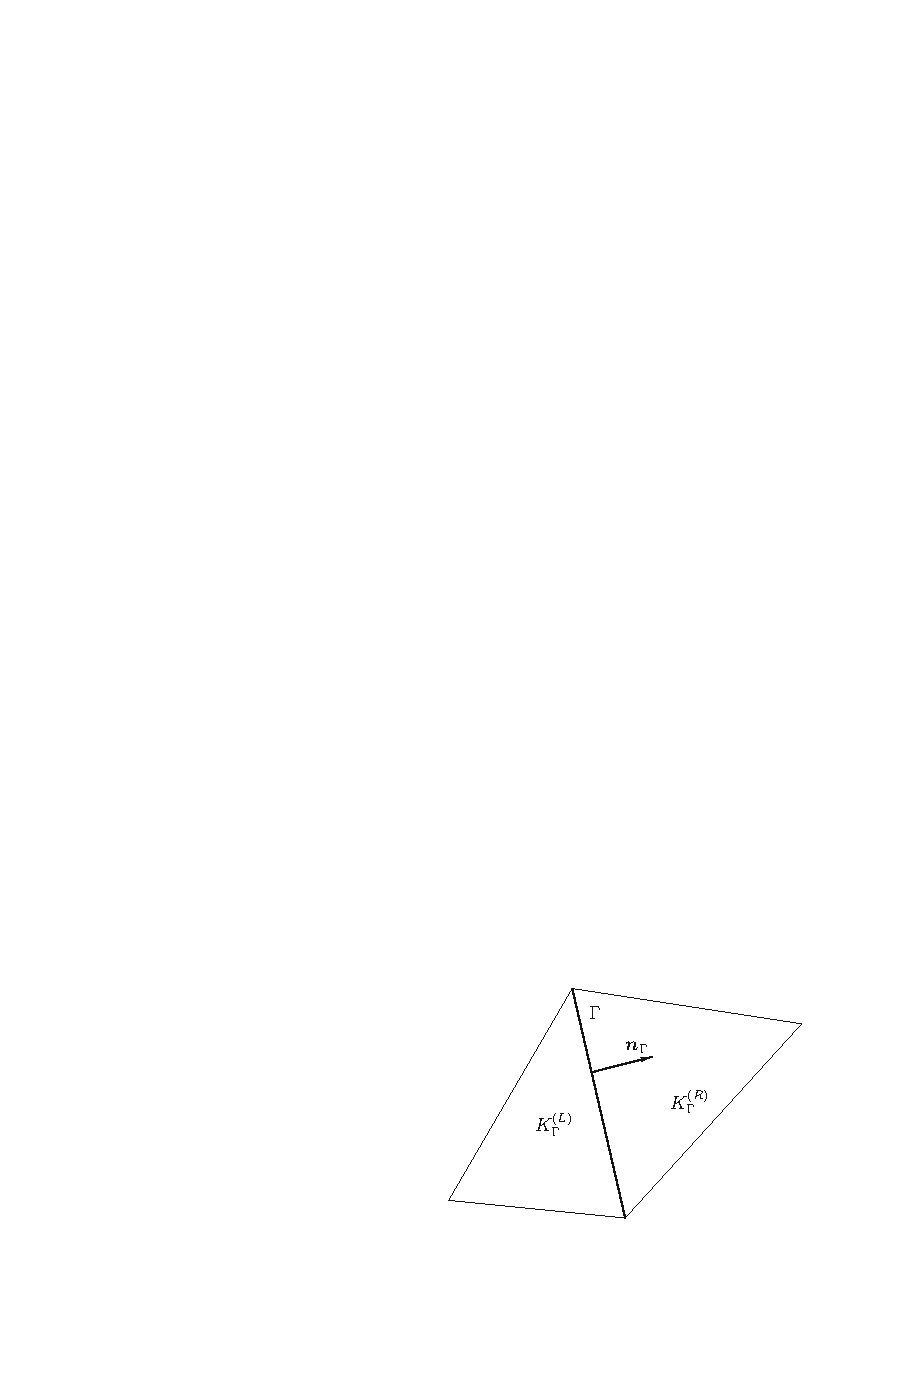
\includegraphics[totalheight=2in]{LR1}
\end{center}
According to \eqref{relation}, the $(\mathbb Q^T, \mathbb U^T)^T$  can be expressed with $\bf\Lambda$, so it lead to a linear system of equations, Denote by
\begin{equation*}
  \mathbb{K}\hat{\bf{U}}  = \bf{L}
\end{equation*}
where $\hat{\bf{U}}$ is the unknowns consist of $\bf\Lambda$ from every element.Suppose ${\bf \Lambda}_{i}$ is one of the $\bf\Lambda$ derived from i-th element, We have
$\hat{\bf{U}} = [{\bf \Lambda}_{1}^T,{\bf \Lambda}_{2}^T,\cdots {\bf \Lambda}_{\mathscr N}^T]^T$.

\subsection{assemble $\mathbb{K}$}
On elements $K$, We known \eqref{1last} origin from
\begin{equation*}
  \big\langle\hat{\bf q}_h\cdot{\bf n}, m_{\Gamma}^i\big\rangle_{\partial K}, \qquad \Gamma \in \partial K
  ,\quad i = 1,2,\cdots \mathscr N_{bp}
\end{equation*}
i.e.
\begin{equation*}
  \sum_{\Gamma \in \partial K} \big\langle\hat{\bf q}_h\cdot{\bf n}, m_{\Gamma}^i\big\rangle_{\Gamma}
  := \mathbb{X}{\bf\Lambda} - {\bf Y} , \qquad \Gamma \in \partial K
  ,\quad i = 1,2,\cdots \mathscr N_{bp}
\end{equation*}
We can circled with each element, lead to relevant algorithm\\
for $e=0:\mathscr N-1 $ \\%对单元循环   \\
    \hspace*{20pt}for $i=0:\mathscr N_b-1 $  \\%对单元边界循环\\
        \hspace*{40pt}\textbf{for} $k=0:\mathscr N_{bp}-1 $ \\%对边界节点循环   \\
            \hspace*{60pt}$I = \tau(e, i, k)$  \\%算出边界节点的全局编号\\
            \hspace*{60pt}for $j=0:\mathscr N_b-1 $  \\%再对单元边界循环\\
                \hspace*{80pt}for $h=0:\mathscr N_{bp}-1 $ \\%再对单元循环   \\
                    \hspace*{100pt}$J = \tau(e, j, h)$  \\%再算出边界节点的全局编号\\
                    \hspace*{100pt}$\mathbb{K}[I][J] += \mathbb{X}[k+i\mathscr N_{bp}][h+j\mathscr N_{bp}]$ \\
                %做叠加 \\
                \hspace*{80pt}end\\
            \hspace*{60pt}end\\
        \hspace*{40pt}\textbf{end}\\
    \hspace*{20pt}end\\
end\\
Where $\mathscr N$ is the numbers of all elements, $\mathscr N_b$ is the numbers of boundarys of each element ,as triangle element $\mathscr N_b=3$ and rectangle element $\mathscr N_b=4$, $\mathscr N_{bp}$ is the numbers of points in boundary of element. $\mathbb{K}$ is left coefficient matrix of \eqref{flux2}. $\tau$ is the mapping from local boundary index to global boundary index. \\

\subsection{assemble $\bf{L}$}
Similarly with assemble $\mathbb{K}$, We can circled with each element, lead to relevant algorithm\\
for $e=0:\mathscr N-1 $ \\%对单元循环   \\
\hspace*{20pt}\textbf{for} $i=0:\mathscr N_b-1 $  \\%对单元边界循环\\
        \hspace*{40pt}for $k=0:\mathscr N_{bp}-1 $ \\%对边界节点循环   \\
            \hspace*{60pt}$I = \tau(e, i, k)$  \\%算出边界节点的全局编号\\
            \hspace*{60pt}${\bf L}[I] += {\bf Y}[k+i\mathscr N_{bp}]$ \\%做累加   \\
        \hspace*{40pt}end\\
    \hspace*{20pt}\textbf{end}\\
end
\end{document}
